


\subsection{Dynamic Assurance}

\subsubsection{Current Approaches and Issues} 
% Suggested relocation color code: 
%\textcolor{orange}{Move to Overview}
%\textcolor{blue}{Move to TA1}
%\textcolor{cyan}{Move to TA2}

%\begin{itemize}
%\item Briefly describe current approaches
%\item Discuss challenges/issues with these approaches
%\item What makes our approach innovative with respect to the state-of-the-art
%\end{itemize}

% \subsubsection{Current Approaches and Issues}

A recent survey of safety engineering compliance practices relates to our dynamic assurance case  challenge (\cite{RESSJ2013}).  The survey found that practitioners frequently relied upon {\em process-based evidence}, such as verification and validation plans and on safety management plans. When the practitioners provided {\em product-based\/} evidence they provided the requirements specification and test results. The study authors mention their intrigue that evidence types concerning risks and hazards are not among the most frequently reported. 
% Practitioners most often use checklists and expert judgment (with rationale) for assessing evidence.  
Their highest challenge is determining the confidence in evidence supporting a claim about system safety. 
% A critical challenge is gathering the design and development artifacts along with the decision process involved to collect them.  
Formal verification results were used by fewer than 30\% of the study respondents.  Completeness of the evidence is checked {\em manually\/} and through a manual predefined process, according to more than half of the respondents. 

Regarding the structure of an assurance case, it has been popular for many years to refer to legal reasoning and graphical notations (\cite{kelly04}).  
% For small arguments, these graphical notations illustrate how to go about structuring and supporting an argument for the trustworthiness of the system.  
The tree-structured {\em goal structuring notation\/} (GSN) is popular, and its cousin dubbed the {\em claim-argument-evidence\/} is an alternate representation.  
% Again for small arguments, one could question whether these are an improvement over free-form text.  
For larger arguments, the tree structures quickly become undesirable, fine for computer internal representation but clumsy for human-computer interfaces or printed documents.  Moreover, there is no specification for the automated analysis of these trees, leaving the user to impose writing requirements to facilitate analysis (\cite{rushby10}).  Somewhere in-between graphical notations and free-form text is semi-structured text (\cite{CMK08}), a DSL for writing case arguments while lending support for fancy editors and automated analysis.

Interesting assurance case structures that lend themselves to analysis have been developed.  
% We describe here the Resolute language, the Evidential Tool Bus, and the $L$ domain specific language (DSL).  
The Resolute language consists of both a logic and a computational sublanguage (\cite{Resolute}). The logic of Resolute is an intuitionistic logic similar to pure Prolog, but augmented with explicit quantification. 
% The logic is parameterized by the computational sublanguage, and requires only that the sub-language is deterministic. 
% This allows the computational sublanguage to be customized to any domain, such as AADL, and to be expanded and refined, without worrying about the logical consequences.   
The Evidential Tool Bus (ETB) (\cite{ETB}) is similar in syntax and semantics to Resolute. It provides a Datalog-style logic and is designed to combine evidence from a variety of sources. However, the focus of the ETB is on distribution and on provenance.  
% It logs the sequence of tool invocations that were performed to solve a query. 
% It uses timestamps to determine which analyses are out of date with respect to the current development artifacts and to only re-run those analyses that are not synchronized with the current development artifacts. 
% ETB is meant to be tool and model agnostic, and therefore has no particular knowledge of the system architecture.  
The DSL $L$ takes a semi-structured text approach (\cite{CertWareABSA}).  It provides an English-like language having a reasonable syntax and semantics for authors to write cases in an argument structure, but also provides analytic support for the document.  The $L$ tool set provides an answer set solver to reason about the case argument and return results to the author. 


% \subsubsection{Issues with Current Approaches}

The safety practitioner survey revealed that simple textual templates are the most frequently found technique for evidence structuring. Study respondents reported rarely using argumentation-based graphical notation such as goal-structuring notation (GSN) or process models such as the OMG's software and system process engineering metamodel (SPEM).  Regarding argumentation-based graphical notations, the study authors note ``[t]he results suggest that a lot of research effort has been spent on a technique that has seen little industrial adoption thus far''.  We speculate, based on our own experience building tool sets for such graphical models, that the problem of quickly becoming unwieldy when modeling real-world products undermines the appeal of these techniques. 

The notation problem can be addressed by domain-specific languages that enable analysis support.  We introduced {\em answer set programming\/} (ASP) technology to provide this support \cite{CertWareABSA}, illustrating analysis of arguments, but the implementation lacks strong formalisms for handling learning, reasoning about uncertainty, and performance scalability.  Although there are some existing algorithms for learning assurance rules in ASP \cite{ray2009nonmonotonic,athakravi2013learning,law2014inductive,athakravi2015inductive,iled,kazmi2017improving}, they do not work well with large data sets. The best performing among them is the system XHAIL.  For handling uncertainty popular formalisms such as Markov Logic Networks or its recently proposed ASP variant $LP^{MLN}$ do not provide for non-monotonic specification of randomness.  An ASP-specific variant P-log does have the required construct, but lacks in its ability to specify arbitrary weights.  

The LE components introduce unique issues for safety assurance~\cite{SafetyANN}. For example, neural networks lend themselves only to black box analysis but are wanted under verification and validation regimes that require white box analysis.  Hazard analysis cannot be performed in the usual manner owing to the way the network algorithms work.  Implicit, process-based safety assurance is insufficient for neural networks owing to a lack of concern for the functional behaviors of the software.  Explicit, product-based arguments such as proposed herein are more appropriate to consider the functional behaviors. 
% To support the top-level assurance claim for an ANN component we must provide the context for the claim and its support.  The context defines characteristics of the model, appropriate application for the design, and a definition of an {\em acceptably safe\/} threshold. 




\subsubsection{Approach}

\paragraph{Domain Specific Language}

We refer to assurance cases having the conventional structure of a legal argument justifying trustworthiness for the system, in a {\em claim-argument-evidence motif}.  We populate the assurance case differently from most in that we do not use the conventional tree structures.  
% Instead we use declarative observations gathered from the physical system and its requirements,  assumptions, and constraints.  
Our declarative approach employs a DSL as semi-structured text that lends itself to automated analysis.  
We use the design and verification content to populate the assurance case argument for safety property claims and evidence at build-time, coupled with run-time monitors produced alongside the evidence to be checked during operation.  Both the build-time evidence and the production evidence in the learning-enabled environment integrate with the dynamic assurance case to maintain the argument for the trustworthiness of the system.  

We will enhance an existing assurance case DSL called $L$. The DSL works in conjunction with an answer set program (ASP) solver to check assurance case arguments.  We choose ASP technology here over other solvers such as SAT or SMT because, after grounding or translation, it provides better access modeling and specialization opportunities for domain-specific scalability.  When the dynamic argument solution shows that trustworthiness can no longer be established, the the answer set solution will show the conflict by way of admitting multiple models.   We bring the language, the editors, and solvers forward as our starting point for our dynamic assurance case (DAC) implementation.

Leveraging our systems-theoretic approach to design and implementation, we reason about the essential elements of {\em intent\/} and {\em state\/} in the DAC.  Our DAC focuses on reasoning about the states of the system because these states are essential for understanding and managing the constraints imposed for LE-CPS safety.  Moreover, through the DAC we adorn the states with associated design contracts, safety constraints, assumptions, intentions, and interactions among the states.  
% Each state is a template consisting of a state variable history, an estimator, a controller, and if interacting with the world a hardware adapter. While normally such a template facilitates methodical design activities, we adopt it for DAC elements as well.  
For human interaction and debugging, when we provide system design intent in terms of state we can use this information from the DAC to support diagnostic explanations.  The current $L$ language resembles a blend of English and Prolog, and we provide editor support to emphasize ease of use.  


% As an example consider a sample assurance case fragment (Figure~\ref{fig:ta3:tc}) from an $L$ argument for design tool chain verification with the goal of claiming certification credit~\cite{FACTS16}.  The case author proceeds from a high-level risk specification ({\tt invalidity\-Risk}) to refine the many instances (e.g. {\tt mitigated} and {\tt verification\-Risk}) involved in the argument.  
% \begin{figure}[tbp]
% \lstset{language=Prolog}
% \begin{lstlisting}
% invalidityRisk(certification(property P, software S)) if
% 	reliesOn(certification(P,S), evidence E) and 
%     produces(toolChain TC, E, P, S) and
%     verificationRisk(risk R, P, S, TC) and
%     not mitigated(R, P, S, TC).
    
% verificationRisk(unsound(modelChecker), property P, software S, toolChain T) if
% 	modelOf(S, model M) and
%     executes(modelChecker MC, input(P, M), output(verified), T) and
%     produces(T, evidence E, P, S) and
%     includes(E, verified(P, M, MC)).
    
% mitigated(unsound(modelChecker), property P, software S, toolChain T) if
% 	modelOf(S, model M) and
%     executes(modelChecker MC1, input(P, M), output(verified), T) and
%     executes(modelChecker MC2, input(P, M), output(verified), T) and
%     MC1 != MC2.

% type modelChecker = {modelChecker1, modelChecker2}.
% type risk = {unsound(modelChecker)}. 
% ...
% \end{lstlisting}
% \caption[Fragment listing of $L$ tool chain argument]{A fragment assurance case listing written in the $L$ domain-specific language. }
% \label{fig:ta3:tc}
% \end{figure}

\begin{wrapfigure}{R}{0.6\textwidth}
\vspace{-30pt}
% \begin{figure}[tbhp]
\begin{center}
% 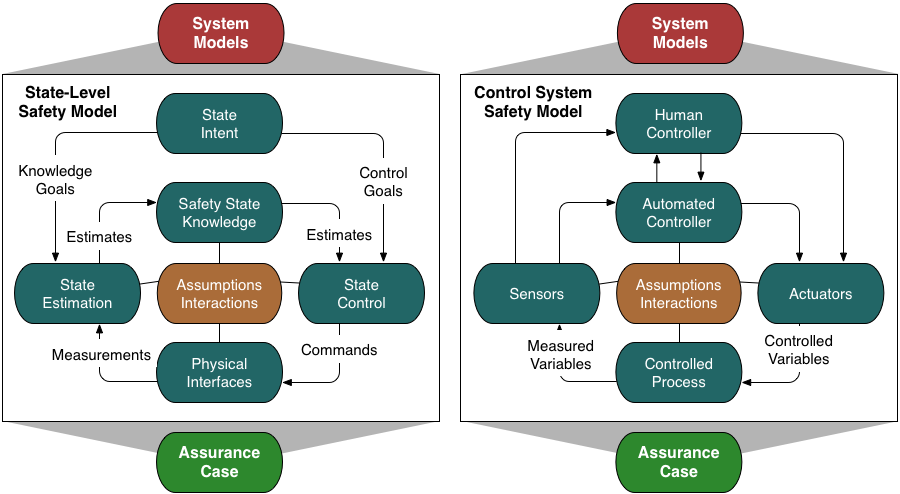
\includegraphics[width=0.8\textwidth]{system_model}
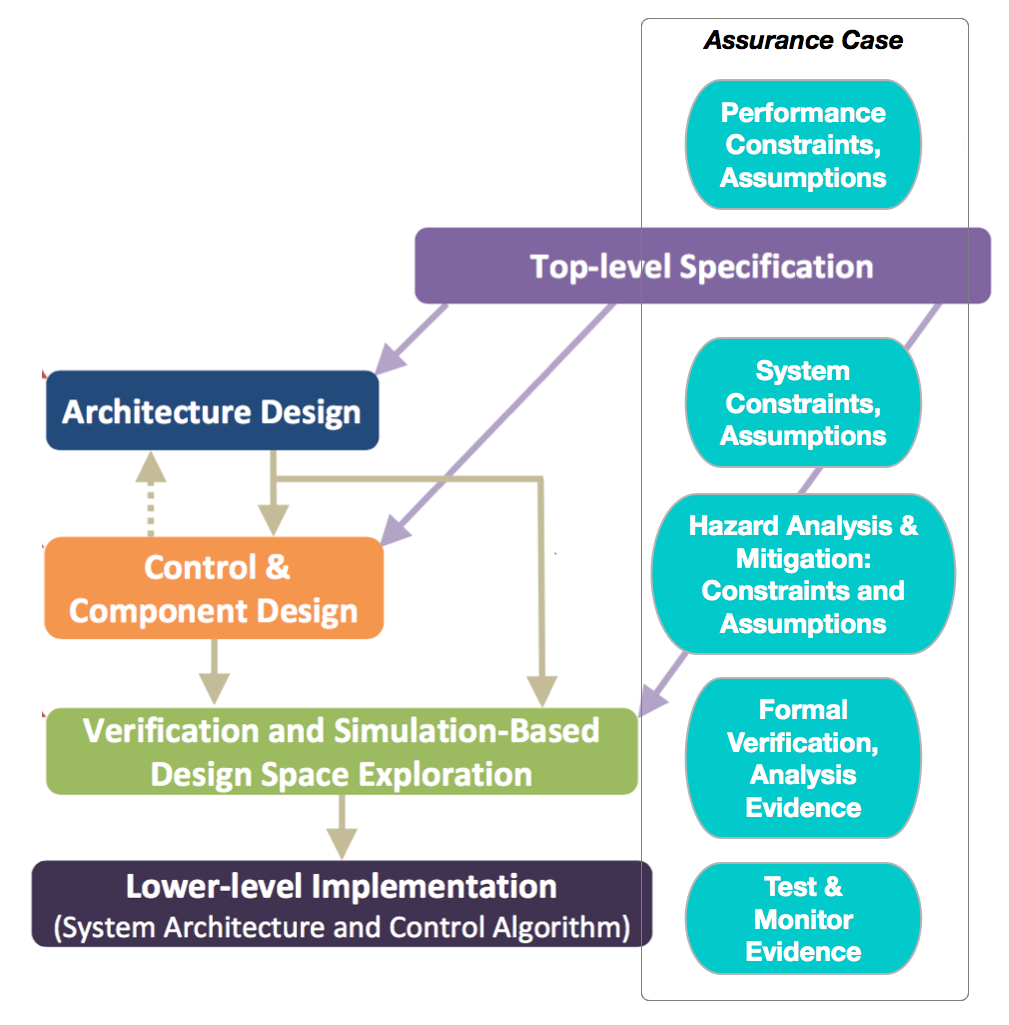
\includegraphics[width=0.6\textwidth,trim={0in 0.2in 0in 0in},clip]{./TA3/dac-sources}
\end{center}
\caption[Assurance case sources]{The system design and runtime activities provide different kinds of content, at different levels of abstraction or refinement, to the dynamic assurance case. }
% \caption[Assurance case sources]{System safety models at different levels of abstraction.  For the state model, instantiations of the pattern for each system state help to specify the system models and to communicate system safety data to the assurance case.  For the system model, control loops around a controlled process help capture the design constraints for the DAC.  } 
\label{fig:statemodel}
% \end{figure}
\vspace{-25pt}
\end{wrapfigure}

\paragraph{Assurance Solver Implementations}

We will improve one or more reasoning engines for our DAC DSL to improve their suitability for dynamic assurance.  There exists several excellent inference engines for basic ASP. 
These include Clingo~\cite{clingo} and Potassco~\cite{potassco}, smodels~\cite{smodels}, and DLV for basic ASP and some systems for languages such as P-log and $LP^{MLN}$ that augment ASP with probabilities and weights. We anticipate building specialized solvers, rather than general-purpose solvers, to support our goals for the program. 

\noindent\underline{Supporting Learning}

During Phase I, we will modify $L$ to accommodate learning of assurance rules.  To have a common formal representation of various modules and components of the learning enabled autonomous systems, we aim to develop learning enabled components that can be characterized using the common representation. 
% For a seamless integration we aim to develop tools and algorithms that can learn rules in ASP and $L$ from data. 

The general sub-area of learning logic rules from data is called inductive logic programming (ILP). 
In statistical machine learning, it is common to learn a function from a series of $\langle x, y \rangle$ pairs where $x$ denotes the input and $y$ denotes the desired output. On the other hand, ILP deals with learning a logic program $H$ given some background knowledge and a dataset containing positive and negative examples. More formally, Given a set of positive examples $E^{+}$, negative examples $E^{−}$ and some background knowledge $B$, an ILP algorithm \cite{muggleton1991inductive} finds a hypothesis $H$ such that, $B \cup H  \models E^{+}$, $B \cup H \not \models E^{−}$. The possible hypothesis space is often restricted with a language bias that is specified by a series of mode declarations $M$.

Because of the mismatch between statistical machine learning and ILP definitions, one needs to convert all the $\langle x,y \rangle$ to create a global $E^{+}$ and $E^{−}$ and extra care needs to be taken so that different $\langle x,y \rangle$   pairs do not interfere with each other.  This approach fails to scale up. That is because, when we have a large  number of $\langle x,y \rangle$  pairs, the ILP solvers will then have to deal with large ASP programs,  We propose to develop a novel iterative and incremental approach where instead of making the above conversion, the learning of rules is done by iteratively going over each example $\langle x,y \rangle$ pair.   Our approach is based on {\em context dependent learning}. By changing the inductive logic programming paradigm to context dependent learning, we will be avoiding dealing with large examples that is made of combining the set of examples. This allows us to pursue an iterative and incremental approach making our approach scalable.  We expect an order of magnitude or more improvement. 
% In this formulation, each example $E_i$ directly corresponds to an $\langle x,y \rangle$ pair and it takes into account that there are several distinct examples in a dataset. 
%We aim to develop an algorithm that will find the solutions incrementally. First it will compute the solutions of $ILP^{ctx}(\langle B,M,{E_1}\rangle)$, then it will use those to find the solutions $ILP^{ctx}(\langle B,M,{E_1, E_2} \rangle)$ and so on until it finds a solution for the original problem, $ILP^{ctx}(\langle B,M,{E_1,...E_n}\rangle)$. Thus, our algorithm will not compute the solutions of $ILP^{ctx}(\langle B,M,{E_1, E_2,..E_i}\rangle)$ in a single step. Rather it will compute several lower bound-upper bound pairs on the search space and employ a state space search for each lower bound-upper bound pair until all the minimal solutions in that space are found. 


% , defined as follows:
%{\bf Definition}:	A \textit{Context Dependent Learning} task $ILP^{ctx}$ is a tuple $\langle B,M,D \rangle$, where $B$ is an Answer Set Program, called the background knowledge, $M$ defines the set of rules allowed in hypotheses (the hypothesis space) and $D$ is the dataset containing a series of context dependent examples $E_1,E_2,..., E_n$. Here each $E_i$ is a tuple $\langle O_i,E_{i}^{+}, E_{i}^{-} \rangle$ where,  $O_i$ is a logic program, called \textit{observation} , $E^{+}$ is a set of positive ground literals and $E^{-}$ is a set of negative ground literals. A hypothesis $H$ is an inductive solution of $T$ (written as $H \in ILP^{ctx}(B,M,D)$) \textit{iff}
%	$H\cup B \cup O_i \vdash E_{i}^{+}, ~\forall i=1...n$,  and   
%	$H\cup B \cup O_i \not \vdash E_{i}^{-}, ~\forall i=1...n$. 

Another learning aspect we will address is allowing previously undefined predicates in $H$. Currently, in all ILP systems and algorithms the mode definitions of rules in $H$ do not allow previously undefined predicates. 
% However, such predicates are needed to learn rules whose conditional part may contain universal quantifications. 
The universal quantification plays an important role in the specification of temporal operators ``{\em always\/}'' and ``{\em until\/}''.

\noindent\underline{Supporting Uncertainty}

During Phase II, we will add support for uncertainty. 
%In recent years several extensions of ASP have been proposed to account for uncertainty.  One approach, as used in P-log, enhances ASP with some explicit probability assignments and additional implicitly derived probability numbers. In another approach, as used in LP\^MLN (and even in the much earlier introduced ASP with weak constraints), weight assignments are given explicitly and probability numbers are computed on top of them.  
We propose to develop a new formalism that incorporates reasoning features crucial to assurance with respect to autonomous systems, such as causality, counter-factual reasoning, use of weights for computing probabilities, 
% instead of direct probability numbers, which are hard to estimate for assurance rules) from which probabilities are computed, 
and probabilistic non-monotonicity -- the ability to have new possible models as a result of new information. 
Probabilistic non-monotonicity is useful for non-\naive\ conditioning, as \naive\ conditioning may fail with new sensors that ask different kind of questions and as a result need a new set of possible worlds \cite{halpern2003, baral2007}. 
% (Such a situation is described in \cite{halpern2003} and addressed in the context of ASP by us in \cite{baral2007}.) 

%To allow non-\naive\ conditioning we need rules of the form:
%\begin{equation*}
%{\tt random}(o(Y) : \{X : p(X)\}) :- a_1, \ldots , a_n, \ {\bf not} \ b_1, \ldots, \ {\bf not} \ b_m. 
%\end{equation*}
%The above rules state that $o(Y)$ is a random variable where $Y$ can take the value from the set \{X : p(X)\} when $B$ is true. Such a construct allows non-monotonic specification of when $o(Y)$ is a random variable and what its extent is. Such non-monotonic specification of randomness is not possible in the popular uncertainty formalisms such as Markov Logic Networks or its recently proposed ASP variant $LP^{MLN}$. While P-log has such a construct, it lacks in its ability to specify arbitrary weights. 

\noindent\underline{Supporting Scaling}

During Phase III, we will focus on ASP solver speed improvements.  There exist excellent inference engines for basic ASP, but none of them has emphasized speed.  We will develop a more efficient system by modularizing the ASP programs and making domain-specific restrictions on the modules.  

Fortunately, we have many innovative ideas for improving the performance of such solvers by several orders of magnitude. Our ideas are derived from the state-of-the-art techniques developed by our teammate for solving Weighted Constraint Satisfaction Problems (WCSPs). 
% The success of most solvers for basic ASP is derived from that of SAT solvers. As a consequence, 
The WCSP serves as a substrate combinatorial problem for ASP augmented with probabilities and weights. In addition, the WCSP is representationally powerful enough to capture many other combinatorial problems in probabilistic reasoning. We have developed the state-of-the-art methods for solving WCSPs. We can apply these techniques to solve ASP augmented with probabilities and weights. Our intuitions include:
\begin{itemize}
\item The Constraint Composite Graph (CCG)~\cite{k08,k08a,k16} is a graph associated with a WCSP. It can be constructed in polynomial time.  Solving a WCSP is equivalent to solving the Minimum Weighted Vertex Cover (MWVC) problem on its CCG. 
% The CCG provides the first unifying mathematical framework for simultaneously exploiting the locality of interactions between the variables as well as the exact probabilities and weights in these interactions~\cite{}. Sufficient structure in locality of interactions translates to low tree width of the CCG; and sufficient structure in the probabilities and weights translates to bipartivity of the CCG.
\item The {\em half-integral\/} property of the MWVC problem can be exploited towards a kernelization procedure for the WCSP~\cite{cc08}. We can stage a polynomial-time maxflow algorithm that preprocesses a WCSP and fixes the optimal values of a large number of its variables. The remaining variables constitute the {\em core\/} of the combinatorial problem. 
% Our polynomial-time kernelization procedure is so powerful that on about $1/7^{th}$ of the WCSP benchmark instances, the core turns out to be empty, i.e., the problem instances are solved entirely in the polynomial-time phase of the algorithm without requiring search at all~\cite{}. In general, for the remaining core of the combinatorial problem, we have also developed the state-of-the-art MWVC solvers~\cite{}.
\item Message Passing (MP) is a well known technique used for large scale combinatorial problems~\cite{kf09}. It avoids exponential time complexity and constitutes an anytime algorithm.  It is known to work very well on several inference problems in Information Theory~\cite{yfw03}.
% However, its behavior was not well understood on Probabilistic Graphical Models or WCSPs until recently. In our recent work, 
We have shown that MP applied on the CCG of a WCSP produces solutions of much higher quality compared to MP applied directly on the WCSP~\cite{xu2017}.
\end{itemize}

% The recent ASP competition provides benchmark performance \cite{ASPC6}.  With a fixed problem structure in our DAC it is unlikely the multiple portfolio (algorithm selection) technique employed by ME-ASP would add any benefit for its implementation complexity, perhaps favoring the simpler WASP+DLV approach.  

ASP in general is an NP-complete problem. The stratified subset of ASP is quadratic. By having a modular language that separates the specification to a small non-stratified part and having a specialized solver for stratified ASP, we expect order of magnitude improvement in performance.  A recent work~\cite{cuteri} with similar ideas has shown good initial results. In addition, grounding can be done faster using a parallelized system in a multi-core environment.

Recent ASP competition results \cite{ASPC6} note the apparent performance benefit of domain modeling and specialization.  % They offer ``[t]hese advantages are owed to symmetry breaking, cutting down a vast number of redundant representations of solution candidates, as well as compact formulations, reducing the size of ground instantiations by some order of magnitude.'' 
Because we develop a paired DSL and solver implementation, such techniques are applicable to us for scalability enhancements.  The competition revealed that on decision problems like ours, the fastest general-purpose solvers produced solutions at a rate of $0.2$ problems per second on the reference Linux platforms.  We expect our specialized solvers to well exceed this performance level on our target application.

% the Multi-Engine ASP Solver (ME-ASP) \cite{MEASP} and WASP+DLV technologies performed the best in the competition's single-processor track.  ME-ASP average time on an array of grounded decision and query problems amounted to $0.2$ problems per second on the reference Linux platform.  However, ME-ASP uses algorithm selection to provide general-purpose coverage; our specialized solver should be expected to exceed this performance threshold on its target application.  

\paragraph{Integration and Demonstration}

We envision providing an API for content producers and consumers to use for interacting with the DAC.  Our design and verification tools and run-time monitors and operators will assert assurance argument structures and features by way of the API.  Any DAC control parameters will be done with a separate API.  We envision using a representational state transfer (REST) stateless specification and synthesizing software adapters for this API.  

As an example of high-level safety requirements, we would commence with explicit control system safety claims in our design activity.  A representative set is given in \cite{NPR7150} regarding completeness of requirements for safety-critical software.  These address conditions such as reachability of safe and unsafe states, operator overrides, error handling, and so on.  We will assert these as specific claims under a top-level safety claim for the assurance argument, then propagate the claims through our hierarchical design and hazard analysis procedure.  
% Various levels of abstraction or refinement of the models provide content for the argument, contributing various granularities of claim and evidence for composing the argument.   
% In some cases the design and verification steps will produce corresponding run-time monitors for conditional evidence gathering.  
Verification tools produce monitors to cover the behaviors of the system that could not otherwise be proven correct -- for which more information is needed.  We determine and justify the need for the run-time monitor and its conditional evidence as part of the design.  
Our DAC reasoning engine may be designed in as an integral part of the safety framework, thus having safety requirements of its own in the integrated system.  We will provide all integration support via software installation and API services, and support demonstration planning and conduct as requested. 




\begin{table}
\caption{Project Plan for TA3}
  \centering
  {\footnotesize
\begin{tabular}{|m{.6in}|m{5.55in}|} 
\hline
\textbf{Phase} & \textbf{Plan} 
\\\hline
Phase I & 
We will build the correspondence mechanisms for the safety-verification-monitor checks across the assurance case, focusing on contracts and constraints at various levels of abstraction in the design and implementation.  We update an existing DSL and ASP solver to focus on this LE-CPS application, and build an API for exchanging constructs and data with the DAC.  We show how the reasoning unfolds for successful and unsuccessful events.   
\\ \hline
Phase II & 
We will elaborate on our Phase I activities to include compositional arguments, uncertainty representations, learning-enabled ASP solvers, adjusting DSL, API, and solvers as required for successful demonstration.  We anticipate having more formal verification and monitor data available at different levels of granularity, both with impact to the DSL. Initial efforts for ASP solver speed scale-up will be undertaken.  
\\ \hline
Phase III & 
We will emphasize scale-up with a primary concern for speed. We will implement modular solvers tailored to our domain, runtime environment, and operating constraints. We  anticipate having more formal verification data available from TA1 at different levels of granularity, as well as more monitor types available from TA2, both with impact to the DSL.
\\ \hline
\end{tabular}
}
\label{tab:ta3:plan}
\end{table}

% During Phase I we will build the correspondence mechanisms for the safety-verification-monitor checks across the assurance case, and show how the case reasoning unfolds for both successful and unsuccessful events.   During Phase II we will expand these techniques to compositional arguments for multiple components acting together to comprise the system.   During Phase III we will further expand to include static analysis correspondence between source and binary images, and including results from dynamic analysis for other properties of interest to the assurance case.  


% note use of enumitem package and [leftmargin=*] to eliminate itemize indentation
\begin{table}
\caption{How TA3 Interfaces with TA1 and TA2}
  \centering
  {\footnotesize
\begin{tabular}{|m{.5in}|m{5.65in}|} 
\hline
\textbf{TA3 } & \textbf{Interfaces and Interaction} 
\\\hline
 TA1 & 
\begin{itemize}[leftmargin=*,topsep=3pt]
\setlength\itemsep{0em} 
%\setlength\parskip{0em}
%\setlength\parsep{0em}
\item Receive assurance-related content in the form of contracts, assumptions, and safety constraints.  Additional information such as  bounds for any learning conducted within the assurance case itself.  Much of this content becomes claims for the assurance case argument.   
\item Receive content in the form of property specifications, open and closed proof obligations, assumptions, interactions, and constraints that led to those results.  
\item Specify and implement an API for the assurance platform which accepts formal verification, simulation, and system testing claims along with assurance case. 
\end{itemize}
\\ \hline
TA2 & 
\begin{itemize}[leftmargin=*,topsep=3pt]
\setlength\itemsep{0em}
\item To support moving evidence into the DAC, TA3 will specify and implement an API for the assurance platform that can receive evidence, conditional evidence, and supporting data.  
\item Evaluate DACs and provide assurance measure when conditional evidence is received. 
\item To support visualization and logging, TA3 will provide an API and services for run-time monitoring of the DAC.
\item To support operational integrity, the design may require fault tolerance for DAC services.  TA3 will provide features for checkpoints, redundancy, roll-backs, or other integrity features. 
\end{itemize}
\\\cline{1-2}
\hline
\end{tabular}
}
\label{tab:ta3:if}
\end{table}




\begin{table}
\caption{Technical Challenges and Mitigation Approach for TA3}
  \centering 
{\footnotesize
\begin{tabular}{|m{1.3in}|m{4.85in}|} 
\hline
\textbf{Challenge} & \textbf{Mitigation Approach} 
\\\hline

Hazard analysis data volume  & 
The ASP technology we use for DAC can easily accommodate large volumes of data.  The ASP reasoning technique enables filtering the results into easily contrasted outcomes so that the practitioner can identify conflicts.\\ \hline

DAC design and implementation validity & 
We consider validation from four perspectives: {\em construct validity\/} (on the theory of DAC and its implementation), {\em conclusion validity\/} (claims to evidence), {\em  internal validity\/} (causal or logical relationships within an argument), and {\em external validity\/} (generalization of results).  
\\ \hline

Identifying sources of verification errors &
Potential sources of verification errors include: modeling errors; testing harnesses and stubbed behaviors; property specification errors; incomplete test results; interpretation (assumption) errors; soundness vs. completeness inference errors in formal methods; artifact misinterpretation or corruption; and tool configuration managements and operation errors. To mitigate these risks we impose assurance arguments on our tool chains.  
\\ \hline

ASP solver speed improvement by specialization to application &
Some expectation of availability and reliability of the DAC application will be imposed by the runtime environment. The challenges are accelerating the ASP solvers and handling time synchronization across multiple DAC instances.
% ; handling fresh and stale data mix; data service drops or corruption; handling defaults in the absence of data; recovery after stop; managing human intervention; and service degradations. 
We explore multiple forms of modular and potentially translated implementations.  
We incorporate the DAC into the system design, potentially including hard real-time and safety downmode features. \\ \hline
\end{tabular}
}
\label{tab:ta3:risk}
\end{table}


